\documentclass{article}
\usepackage[english]{babel}
\usepackage[utf8]{inputenc}
\usepackage{fancyhdr}
\usepackage{amsmath}
\usepackage{amssymb}
\usepackage{amsthm}
\usepackage{geometry}
\usepackage{titlesec}
\usepackage{float}
\usepackage{svg}
\usepackage{listings}
\usepackage{graphicx}

\setcounter{section}{-1}
\title{Poker Guide}
\author{AlgoPoker}
\begin{document}
\maketitle
\tableofcontents
\newpage 
\section{Introduction}
This document will serve as a guide on the rules of poker for use when building a bot for AlgoPoker. We'll first start with the rules of poker, and then move into some basic and deeper strategy, along with suggestions on how to implement these strategies into your bots. The poker type we'll be discussing is "No-Limit Texas Hold-Em", which is the most popular and common variant of poker.
\section{Basic Rules of No-Limit Texas Hold-Em Poker}
No-Limit Texas Hold-Em Poker is a game where players wager chips on strengths of poker hands they hold, with the objective of earning as many chips as possible. Players bet into a pot in several rounds, and the pot is won by a player when everyone else gives up ('\emph{folds}') or they have the best hand at the end of the final round. Players play in a fixed clockwise order in a hand; the player that goes first rotates every hand. 
\subsection{Betting rounds and structure of the game}
In one betting round, the first player either bets nothing ('\emph{check}') or they can bet any amount between the "\emph{big blind}" (more on this later) and the amount of chips they have got left (hence "No-Limit"). Action then passes to the next player. If the first player has bet any amount, the next player can either \emph{fold} (put no more money in and exit the hand), \emph{call} (match the first player's bet), or \emph{raise} (bet more than the first player). If the first player has checked, the second player also has the option to check. If there are more than two people playing, we then move onto the next player who must also at least match the current bet.\\\\
The first betting round has a particular quirk where two players are forced to put in a bet: the \emph{big blind}, which is a fixed amount that this player (who we also call the big blind) must put into the pot. The player to the right of the big blind is called the \emph{small blind} and is also forced to put in a bet half the size of the big blind's.\\\\
The structure of a hand is as follows: the game begins with each player receiving two (secret and unique) hole cards. The first betting round takes place, and then the "\emph{flop}" (three community cards are revealed). After another betting round, there is the "\emph{turn}" (a fourth community card is revealed). Another betting round occurs, and there is the "\emph{river}" (a final fifth community card is revealed). The last betting round takes place next, followed by settlement (cards are revealed and the pot given to the winning player).
\subsection{Hand rankings and winning a hand}
So how does the best hand get decided? After the fifth community card has been revealed, your hand is the combination of five cards out of the five community cards and your two hole cards that ranks the highest out of all of the combinations shown below (the best hand being shown at the top):
\begin{figure*}[h]
    \centering
    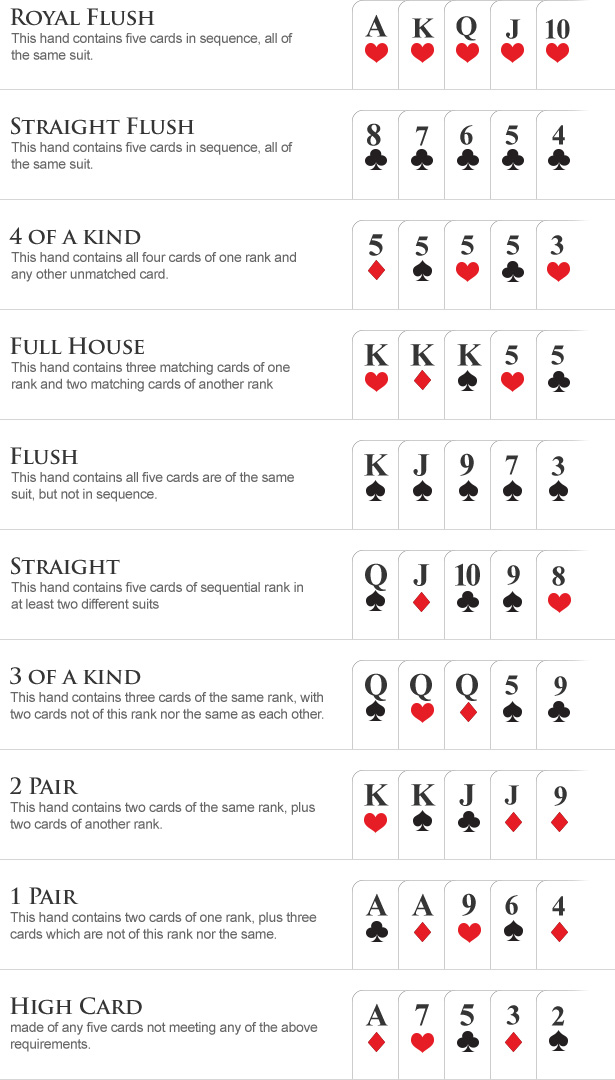
\includegraphics[width=115mm]{how-to-ranking.jpg}
\end{figure*}
\end{document}
